\documentclass[10pt,pdf,hyperref={unicode}]{beamer}
\usepackage[T2A]{fontenc}       %поддержка кириллицы
\usepackage[utf8]{inputenc}   %пока бибтех не дружит до конца с юникодом
\usepackage[russian]{babel}     %определение языков в документе
\usepackage{amssymb,amsmath}    %математика

\usepackage{caption}
\usepackage{subcaption}

\usepackage{float}
\floatstyle{boxed}
\restylefloat{figure}

\usetheme[]{Berlin}
\usecolortheme{rose}

%%%%%%%%%%%%%%%%%%%
%% Выбор шрифтов %%
\usefonttheme[onlylarge]{structurebold}

% Привычный шрифт для математических формул
\usefonttheme[onlymath]{serif}

% Более крупный шрифт для подзаголовков титульного листа
\setbeamerfont{institute}{size=\normalsize}
%%%%%%%%%%%%%%%%%%%

% Если используется последовательное появление пунктов списков на
% слайде (не злоупотребляйте в слайдах для защиты дипломной работы),
% чтобы еще непоявившиеся пункты были все-таки немножко видны.
\setbeamercovered{transparent}

%%%%%%%%%%%%%%%%%%
%%% Сокращения %%%
% Синий цвет выделения
\setbeamercolor{color1}{bg=blue!60!black,fg=white}
%%%%%%%%%%%%%%%%%%

\title{Построение, анализ и оптимизация динамического потока данных в однородной распределенной среде}
\author{Борисяк Максим}
\institute{МФТИ (ГУ)
}
\date{
    \\
    2013г.
}

\newcommand{\stock}{\text{STOCK}}
\newcommand{\source}{\text{SOURCE}}
\newcommand{\initial}{\text{INITIAL}}
\newcommand{\nontrivial}{\text{NON-TRIVIAL}}
\newcommand{\map}{\text{MAP}}

\newcommand{\FA}{F\!A}

\begin{document}
\begin{frame}
  % создаём титульный лист
  \maketitle
\end{frame}

\section{Введение}

\begin{frame}
  \frametitle{Цели работы}
 \begin{columns}
    \column{\textwidth}
     \begin{itemize}
        \item Создание формальной модели потока данных
        \item Анализ неопределенностей в схемах потоков данных
        \item Оценка необходимых ресурсов для запуска потока данных
    \end{itemize}
\end{columns}
\end{frame}

\begin{frame}
  \frametitle{Определение потока данных}
  Поток данных --- модель представления вычеслительных процессов, включающая:
  \begin{itemize}
    \item набор атомарных функций-исполнителей,
    \item составные исполнители или подпотоки данных,
    \item описание зависимостей между исполнителями,
    \item стратегия выполнения.
  \end{itemize}
\end{frame}

\begin{frame}
  \frametitle{Задачи потоков данных}
  \begin{itemize}
    \item Научные-инженерные задачи.
    \begin{itemize}
      \item Большие объемы данных.
      \item Выполнение в распределенных средах.
    \end{itemize}
    \item Изолиция от технических аспектов вычислений.
    \item Отказоустойчивость.
  \end{itemize}
\end{frame}

\begin{frame}
  \frametitle{Приемущества потоков данных}
  \begin{itemize}
    \item Возможность интуитивно понятного визуального представления.
    \item Изолированность от технических аспектов вычислительной среды.
    \item Простота создания.
  \end{itemize}
\end{frame}

\begin{frame}
  \frametitle{Способы представления}
  \begin{itemize}
    \item Декларативные либо скриптовые ЯП.
    \item Графы.
    \item Сети Петри.
    \item Сети процессов Кана (для потоковой обработки).
  \end{itemize}
\end{frame}

\section{Используемая модель}

\begin{frame}
  \frametitle{Используемая модель потоков данных}
  Используется представление в виде ориентированного графа.
  Поток данных --- кортеж $c = (B, E, I, O)$:
  \begin{itemize}
    \item набор блоков $B$ --- каждый блок осуществляет преобразование данных;
    \item связи $E$ --- зависимости по данным между входными портами одних и выходными портами других блоков;
    \item $I$, $O$ --- наборы входных и выходных портов (начальных данных и результатов).
  \end{itemize}
\end{frame}

\begin{frame}
  \frametitle{Блок}
  Блок --- единица преобразования данных, кортеж $s = (\FA, I, O)$:
  \begin{itemize}
    \item $\FA$ --- автомат Мили, описывающий качественное поведение алгоритма блока:
      \begin{itemize}
        \item входной алфавит: $2^I$;
        \item выходной алфавит: $2^O$;
        \item состояния определяют классы внутренних состояний переменных
              алгоритма блока;
      \end{itemize}
    \item $I$, $O$ --- наборы входных и выходных портов.
  \end{itemize}
  Различается два типа блоков:
  \begin{itemize}
    \item атомарные --- предопределенные блоки элементарных операций;
    \item составные --- потоки данных, представленные в виде блоков.
  \end{itemize}
\end{frame}

\begin{frame}
  \frametitle{Наглядное представление блоков и автомата Мили}
  \begin{figure}[H]
  \centering

  \begin{subfigure}[b]{0.2\textwidth}
    \centering
    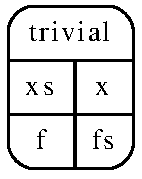
\includegraphics[width=\textwidth]{map_cg.pdf}
    \caption{Схема шаблона \textit{Loop}}
    \label{map:connection}
  \end{subfigure}
  ~
  \begin{subfigure}[b]{0.7\textwidth}
    \centering
    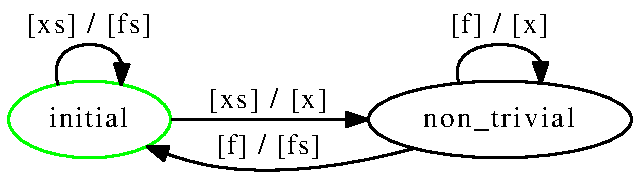
\includegraphics[width=\textwidth]{map_fa.pdf}
    \caption{Автомат Мили шаблона \textit{Loop}}
    \label{map:fa}
  \end{subfigure}
  
  \caption{Схематичное изображение шаблона блока \textit{Loop} (a) и соответствующего ему конечного автомата Мили (b).}
  \label{map}
\end{figure}
\end{frame}

\begin{frame}
  \frametitle{Наглядное представление иерархичного потока данных}
  \begin{figure}[H]
    \centering
    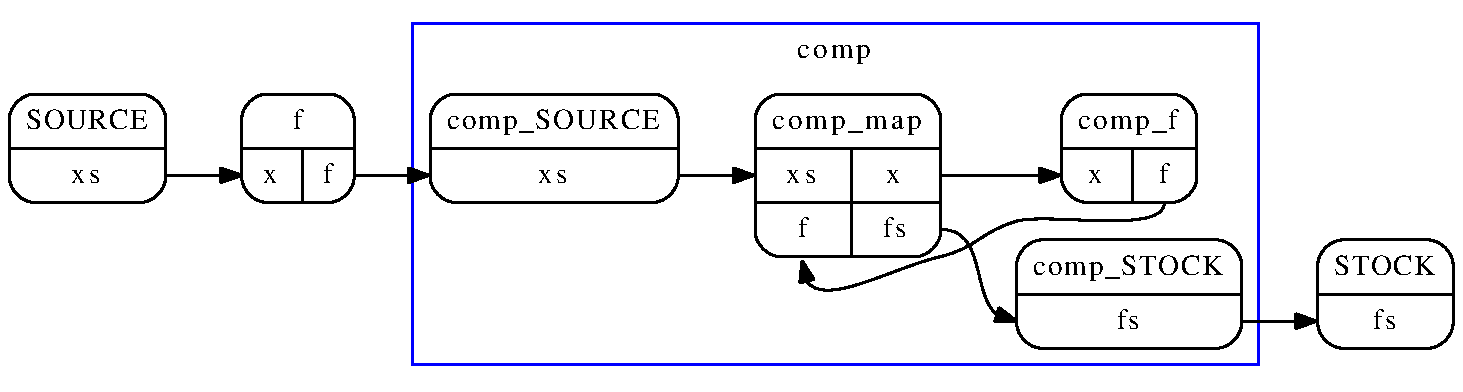
\includegraphics[width=\textwidth]{cc_cg.pdf}
    \caption{Шаблон составного блока. Внутри рамки показана структура шаблона внутреннего блока.}
    \label{example:supercomposite}
  \end{figure}
\end{frame}

\section{Запуск потока данных}

\begin{frame}
  \frametitle{Состояния блока во время запуска потока данных}
  Три состояния каждого блока:
  \begin{itemize}
    \item работает (work) --- выполняет преобразование данных;
    \item заблокирован (blocked) --- завершил работу, но не может испустить данные;
    \item свободен (free) --- не хватает данных для запуска.
  \end{itemize}
  
  \begin{figure}[H]
    \centering
    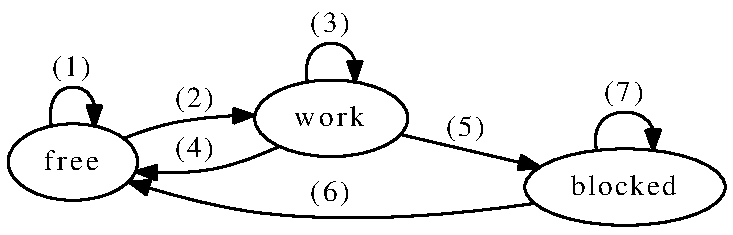
\includegraphics[width=0.9\textwidth]{rules.pdf}
  \end{figure}
\end{frame}

\begin{frame}
  \frametitle{Алгоритм запуска потока данных}
  Алгоритм запуска потока данных:
  \begin{enumerate}
    \item определение блоков для запуска в соответствии с запрашиваемым набором данных \label{check};
    \item передача данных, запуск блоков \label{launch};
    \item проверка возможности вывода блока из состояния 'заблокирован':
      \begin{itemize}
        \item возможно --- переход к шагу \ref{launch};
        \item иначе --- к шагу \ref{wait};
      \end{itemize}
    \item ожидание окончания работы блоков, проверка завершения работы потока данных \label{wait}:
    \begin{itemize}
      \item работа завершена --- окончание, выдача результата;
      \item иначе --- к шагу \ref{check}.
    \end{itemize}
  \end{enumerate}
\end{frame}

\begin{frame}
  \frametitle{Неопределенности в работе потоков данных}
  \begin{itemize}
    \item Варианты переходов автомата Мили блока.
    \item Варианты поглощения данных на входных портах блока.
    \item Состояния гонки: зависимость результата от времен работы блоков.
    \item Остаточные данные и некорректное завершение.
  \end{itemize}
  Первый тип неопределенности --- результат упрощения (детерминированного) алгоритма работы блоков, неопределенности первого рода.
  Остальные --- ошибки построения схемы потока данных, неопределенности второго рода.\\
  \textbf{Корректный поток данных} --- поток данных, не допускающий неопределенностей второго рода.
\end{frame}

\section{Анализ схемы потока данных}

\begin{frame}
  \frametitle{Анализ корректных потоков данных}
  Траектория запуска --- наборы состояний потока данных во все моменты времени. \\
  Граф причинности --- качественное описание варианта поведения потока данных:
  \begin{itemize}
    \item вершины --- кортежи $r = (v, \pi_v, n)$, $v \in B_c$ --- блок, $\pi_v$ --- переход в автомате Мили блока $v$, $n$ - номер.
    \item ребра --- 'причины' запуска: испущенные данные одного блока приняты другим.
  \end{itemize}
  Графы причинности разбивают все возможные траектории запуска на классы эквивалентности.
  Для корректного набора данных каждый класс содержит траекторий соотвующие любым возможным наборам времен работы блоков.
\end{frame}

\begin{frame}
  \frametitle{Простой волновой алгоритм}
  Для ацикличных корректных потоков данных множество графов причинности конечно.
  \begin{enumerate}
    \item проверка на завершенность потока данных:
      \begin{itemize}
        \item поток данных завершен --- возврат графа причинности;
        \item иначе --- далее;
      \end{itemize}
    \item формирование множеств возможных переходов для каждого блока $\{\Pi(v)\}_{v \in B_c}$;
    \item для каждого набора возможных переходов $\{\pi(v) \in \Pi(v)\}_{v \in B_c}$:
    \begin{enumerate}
      \item осуществление переходов $\pi(v)$ c формированием нового состояния потока данных;
      \item дополнение графа причинности;
      \item получение результата рекурсивного запуска из нового состояния;
    \end{enumerate}
    \item возврат объединения результатов.
  \end{enumerate}
\end{frame}

\begin{frame}
  \frametitle{Волновой алгоритм}
  При наличии циклов в потоке данных множество графов причинности бесконечно, но регулярно.
  Волновой алгоритм строит 'внутренний' конечный автомат потока данных --- аналог конечного
  автомата для регулярных языков:
  \begin{itemize}
    \item вершины --- состояния потока данных;
    \item ребра соответствуют работе блоков в потоке данных.
  \end{itemize}
  Циклы соответствуют циклам во 'внутреннем' конечном автомате.
  Любой путь во 'внутреннем' конечном автомате потока данных соответствует графу причинности и наоборот.
\end{frame}

\begin{frame}
  \frametitle{Вероятности на графах причинности}
  Часто используемый пример.
  \begin{figure}[H]
  \centering
  \begin{subfigure}[b]{0.45\textwidth}
    \centering
    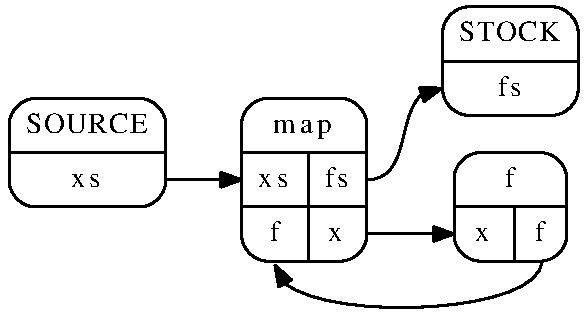
\includegraphics[width=\textwidth]{example_cg.pdf}
    \caption{Поток данных}
  \end{subfigure}
  ~
  \begin{subfigure}[b]{0.45\textwidth}
    \centering
    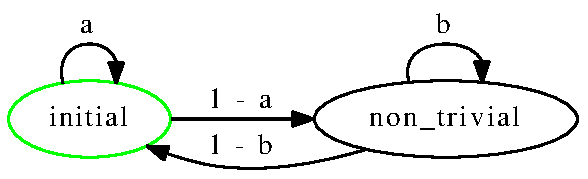
\includegraphics[width=\textwidth]{map_fa_prob.pdf}
    \caption{Автомат Мили шаблона \textit{Loop}}
  \end{subfigure}  
  \caption{Часто используемая схема потока данных}
\end{figure}
$$\mathbb{E}(L) = (1 - a) (1 - b) \sum^{\infty}_{n = 1} n b^{n - 1} = \frac{1 - a}{1 - b}$$
\end{frame}

\begin{frame}
  \frametitle{Анализ графа причинности}
  Выполнение потока данных в однородной распределенной среде.
  Один переход задействует один вычислитель на неопределенное время.\\
  \textbf{Срез графа причинности} $S$ --- множество независимых переходов (задач) графа причинности.\\
  \textbf{Эволюция графа причинности} $\Delta = \{S^j\}^{J}_{j = 0}$ --- набор связанных срезов графа причинности.
  $$N_{\min} = \min_{\Delta} \max_{S^j \in \Delta} \lvert S^j \rvert$$
  $$N_{\max} = \max_{\Delta} \max_{S^j \in \Delta} \lvert S^j \rvert$$
  Выполнять поток данных на $N > N_{\max}$ вычислителях бессмысленно.
  Для $N < N_{\min}$ --- заведомо высокая конкуренция процессов.
  Для определения $N_{\min}$ и $N_{\max}$ используется \textbf{HEFT-алгоритм}.
\end{frame}

\begin{frame}
  \frametitle{Динамическое изменение оценок}
  Все графы причинности образуют префиксное дерево.
  По мере работы потока данных выполняемый граф причинности уточняется --- возможно уточнение оценок.
  Для каждой вершины префиксного дерева можно вычислить $\hat{N}_{\{\max, \min\}, \{\max, \min\}}$ для остатков возможных
  графов причинности.
  Это позволяет осуществить динамическое уточнение оценок необходимых ресурсов.
\end{frame}

\begin{frame}
  \frametitle{Пример потока данных}
  \begin{figure}[H]
    \centering
    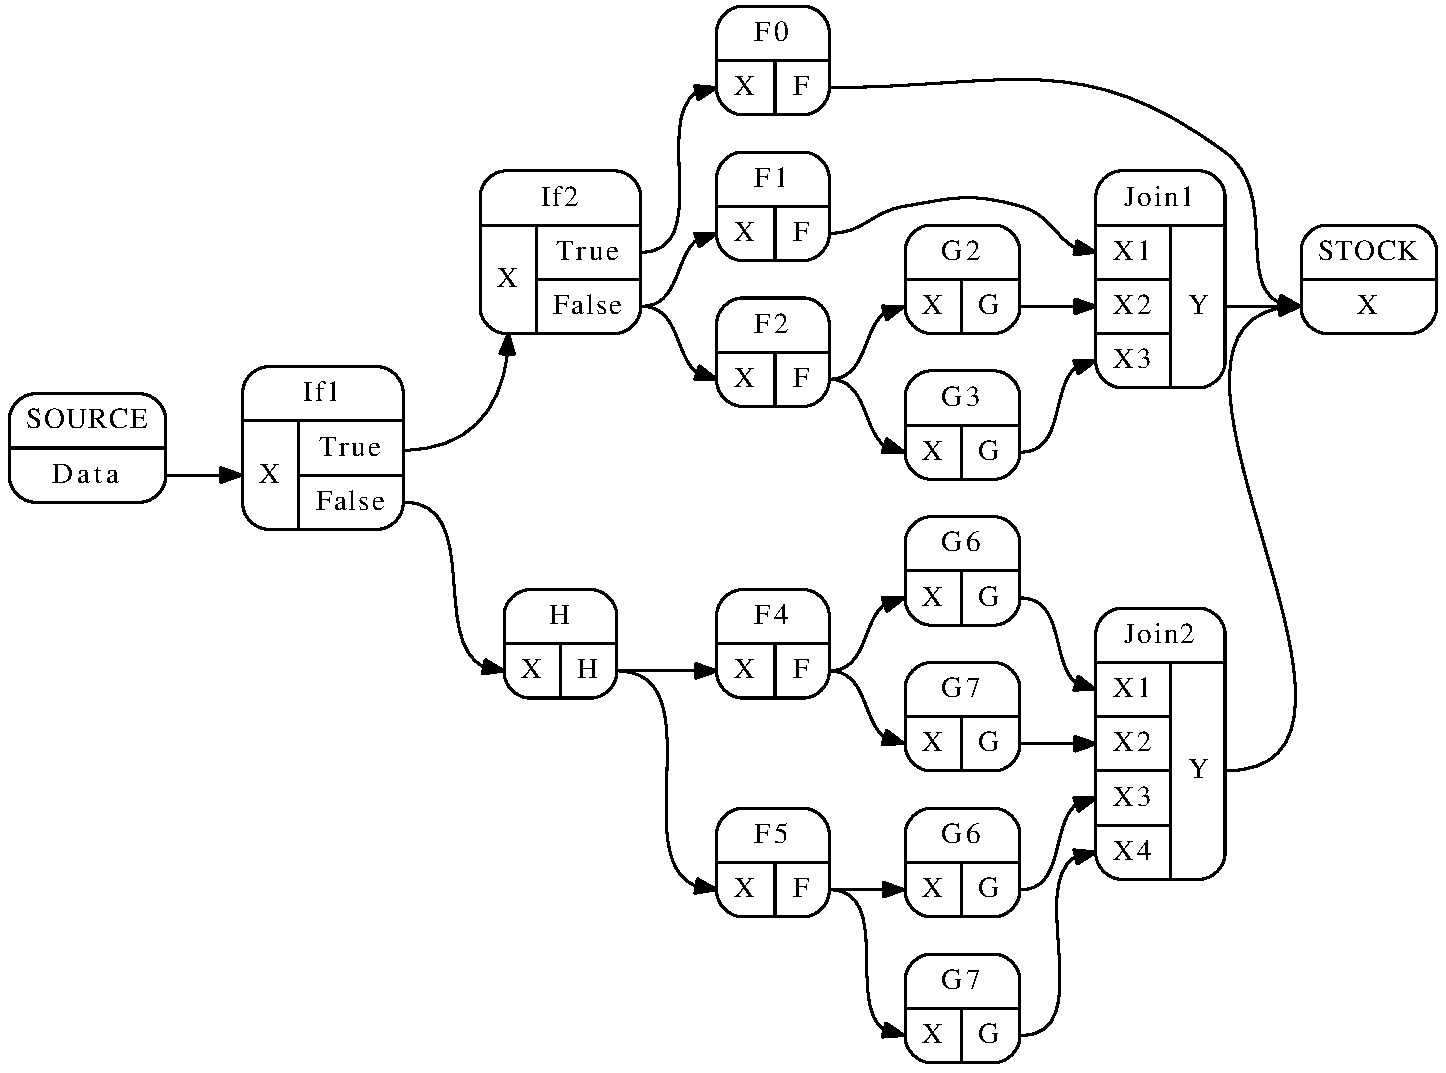
\includegraphics[width=0.75\textwidth]{example2.pdf}
  \end{figure}
\end{frame}

\begin{frame}
  \frametitle{Графы причинности потока данных}
  \begin{figure}[H]
  \centering
  \begin{subfigure}[b]{0.80\textwidth}
    \centering
    
\includegraphics[width=\textwidth]{example2_task_graph_1.pdf}
    \vspace{7pt}
  \end{subfigure}
  ~
  \begin{subfigure}[b]{0.80\textwidth}
    \centering
    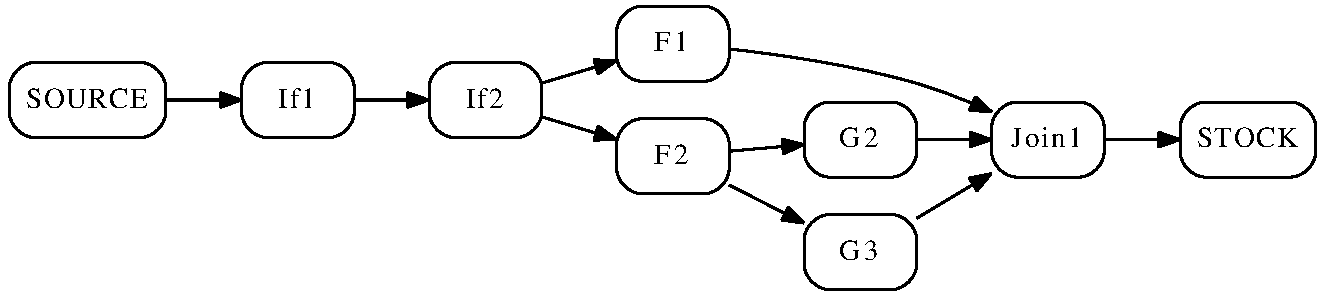
\includegraphics[width=\textwidth]{example2_task_graph_2.pdf}
    \vspace{7pt}
  \end{subfigure}
  ~
  \begin{subfigure}[b]{0.80\textwidth}
    \centering
    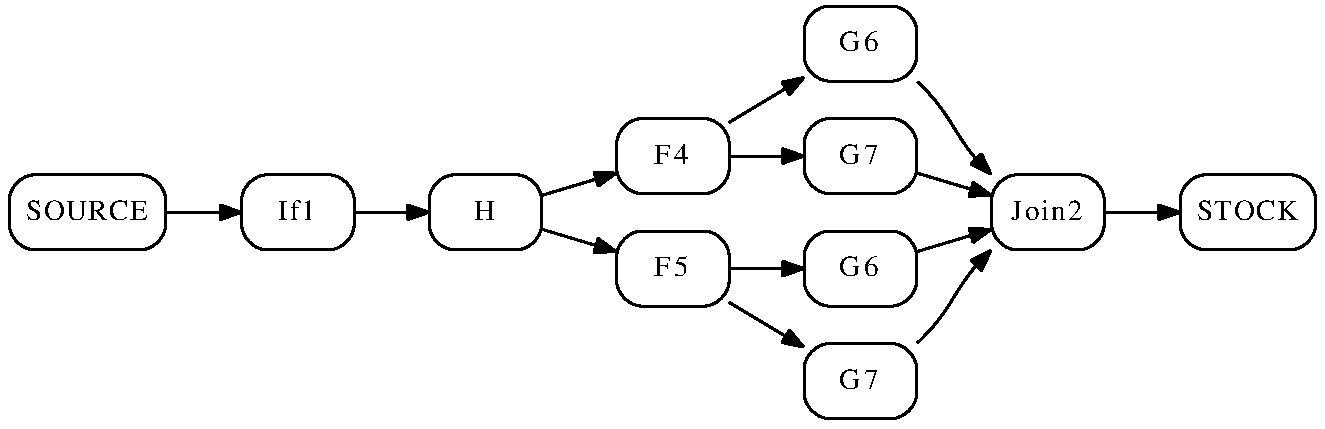
\includegraphics[width=\textwidth]{example2_task_graph_3.pdf}
  \end{subfigure}
  \caption{Три графа причинности потока данных }
\end{figure}
\end{frame}

\begin{frame}
  \frametitle{Результаты динамического уточнения оценок}
  \begin{figure}[H]
    \centering
    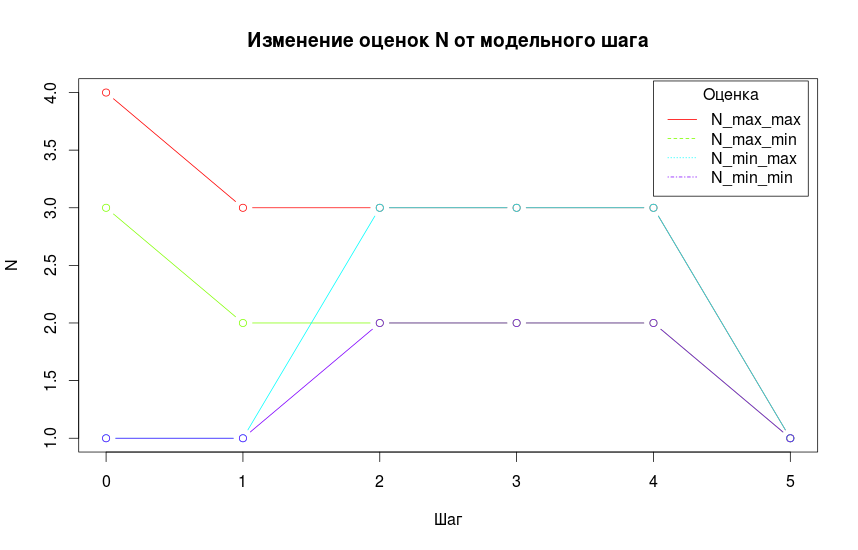
\includegraphics[width=0.9\textwidth]{Rplot01}
    \caption{Динамика изменения оценок в случае 2-го графа причинности}
  \end{figure}
\end{frame}

\begin{frame}
  \frametitle{Обнаружение неопределенностей второго рода}
  \begin{itemize}
    \item Некорректное завершение --- во время работы волнового алгоритма по наличию состояний с остаточным данными.
    \item Варианты поглощения данных --- во время работы волнового алгоритма.
    \item Состояния гонки --- модификация волнового алгоритма.
  \end{itemize}
\end{frame}

\begin{frame}
  \frametitle{Обнаружение состояний гонки}
  \begin{itemize}
    \item \textbf{Коррелирующие волны} --- волны, одна из которых потомок другой.\\
    Модификация волнового алгоритма:
    \begin{itemize}
      \item определение корреляции волн,
      \item ведение истории на портах,
      \item проверка волн при поглощении
    \end{itemize}
 \item \textbf{Детерминированный по входу автомат Мили} $\FA = (S, s_0, \Sigma, \Lambda, E)$:
    $$\forall s \in S: \forall \sigma, \sigma': (s, \sigma, \cdot, \cdot) \in \Sigma \wedge (s, \sigma', \cdot, \cdot) \in \Sigma \Rightarrow \sigma = \sigma'$$
    Такой автомат исключает самый сложный тип состояния гонки --- гонку на различные варианты поглощения.
  \end{itemize}
\end{frame}

\begin{frame}
  \frametitle{Пример с аппроксиматором}
    \begin{figure}[H]
  \centering

  \begin{subfigure}[b]{\textwidth}
    \centering
    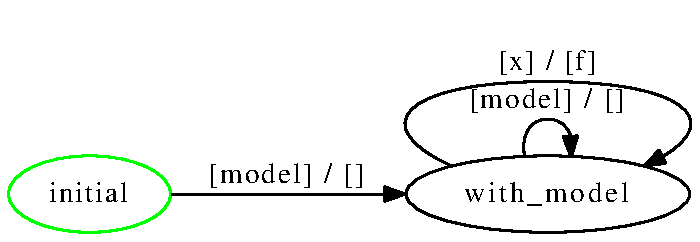
\includegraphics[width=0.8\textwidth]{approx_fa.pdf}
    \caption{Не детерминированный по входу автомат Мили блока аппроксимации}
    \label{notdetFA}
  \end{subfigure}
  ~
  \begin{subfigure}[b]{\textwidth}
    \centering
    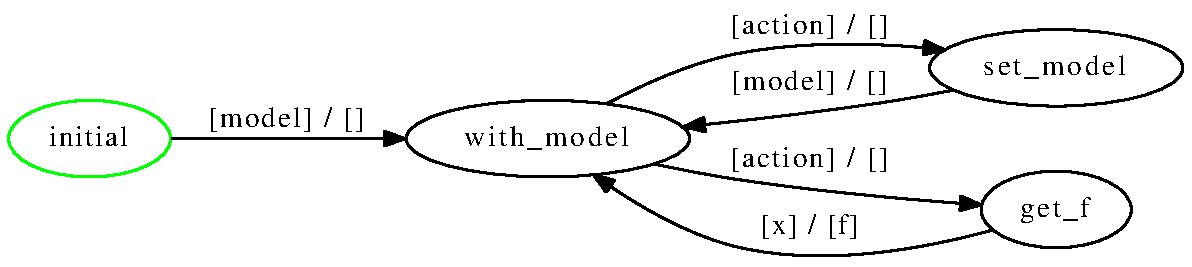
\includegraphics[width=0.8\textwidth]{approx_fa_det.pdf}
    \caption{Детерминированный аналог}
    \label{detFA}
  \end{subfigure}
  \label{det_example}
  \end{figure} 
\end{frame}

\section{Заключение}

\begin{frame}
  \frametitle{Результаты}
  \begin{itemize}
    \item Построена модель потока данных.
    \item Определены возможные неопределенности и ошибки построения потока данных.
    \item Построен алгоритм нахождения ошибок построения потока данных.
    \item Найдены алгоритмы нахождения стратегий запуска для корректных алгоритмов.
  \end{itemize}
\end{frame}

\begin{frame}
  \frametitle{Дальнейшая работа}
  \begin{itemize}
    \item Введение модели оценки времени работы потока данных:
    \begin{itemize}
      \item модель оценок времен работы блоков;
      \item стохастическая модель переходов;
      \item обработка историй реальных запусков методами анализа данных.
    \end{itemize}
    \item Алгоритмы автоматической кластеризации блоков.
    \item Модификация модели потоков данных.
    \item Анализ работы потоков данных в гетерогенных и/или динамических распределенных средах.
    \item Анализ свойств потоков, построенных на основе определенного набора атомарных блоков.
  \end{itemize}
\end{frame}




\end{document}